% Diagrama representativo de la señal cuadrada en tiempo y frecuencia (Consigna pág. 5)
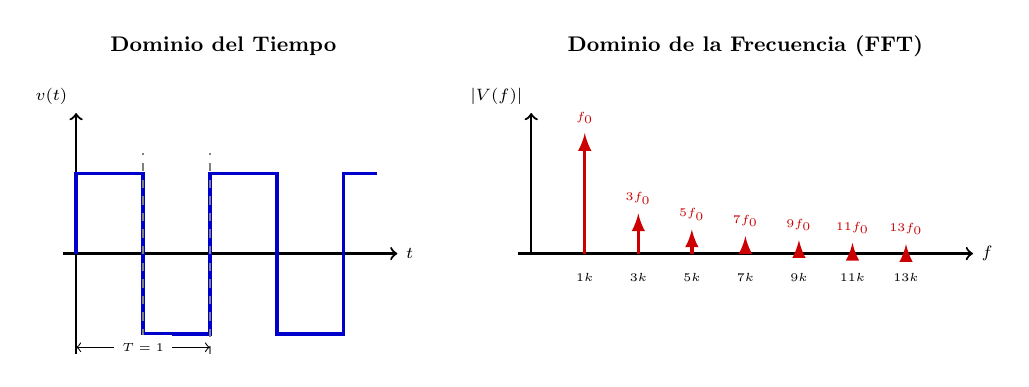
\begin{tikzpicture}[scale=0.85, transform shape]
    % Dominio del tiempo
    \begin{scope}[shift={(0,0)}]
        \node at (2.2, 3.1) [font=\small\bfseries] {Dominio del Tiempo};
        \draw[->, thick] (-0.2,0) -- (4.8,0) node[right, font=\scriptsize] {$t$};
        \draw[->, thick] (0,-1.5) -- (0,2.1) node[above left, font=\scriptsize] {$v(t)$};
        \draw[blue!80!black, very thick] 
            (0,0) -- (0,1.2) -- (1.0,1.2) -- (1.0,-1.2) -- (2.0,-1.2) 
            -- (2.0,1.2) -- (3.0,1.2) -- (3.0,-1.2) -- (4.0,-1.2) -- (4.0,1.2) -- (4.5,1.2);
        \draw[dashed, gray] (1.0,-1.5) -- (1.0,1.5);
        \draw[dashed, gray] (2.0,-1.5) -- (2.0,1.5);
        \draw[<->, font=\tiny] (0,-1.4) -- (2.0,-1.4) node[midway, fill=white] {$T = \qty{1}{\milli\second}$};
    \end{scope}

    % Dominio de la frecuencia (FFT)
    \begin{scope}[shift={(6.8,0)}]
        \node at (3.2, 3.1) [font=\small\bfseries] {Dominio de la Frecuencia (FFT)};
        \draw[->, thick] (-0.2,0) -- (6.6,0) node[right, font=\scriptsize] {$f$};
        \draw[->, thick] (0,0) -- (0,2.1) node[above left, font=\scriptsize] {$|V(f)|$};
        
        % Rayas espectrales impares
        \draw[red!80!black, very thick, -latex] (0.8,0) -- (0.8,1.8) node[above, font=\tiny] {$f_0$};
        \draw[red!80!black, very thick, -latex] (1.6,0) -- (1.6,0.60) node[above, font=\tiny] {$3f_0$};
        \draw[red!80!black, very thick, -latex] (2.4,0) -- (2.4,0.36) node[above, font=\tiny] {$5f_0$};
        \draw[red!80!black, very thick, -latex] (3.2,0) -- (3.2,0.26) node[above, font=\tiny] {$7f_0$};
        \draw[red!80!black, very thick, -latex] (4.0,0) -- (4.0,0.20) node[above, font=\tiny] {$9f_0$};
        \draw[red!80!black, very thick, -latex] (4.8,0) -- (4.8,0.16) node[above, font=\tiny] {$11f_0$};
        \draw[red!80!black, very thick, -latex] (5.6,0) -- (5.6,0.14) node[above, font=\tiny] {$13f_0$};

        % Ticks en el eje
        \node at (0.8,-0.35) [font=\tiny] {$1\text{k}$};
        \node at (1.6,-0.35) [font=\tiny] {$3\text{k}$};
        \node at (2.4,-0.35) [font=\tiny] {$5\text{k}$};
        \node at (3.2,-0.35) [font=\tiny] {$7\text{k}$};
        \node at (4.0,-0.35) [font=\tiny] {$9\text{k}$};
        \node at (4.8,-0.35) [font=\tiny] {$11\text{k}$};
        \node at (5.6,-0.35) [font=\tiny] {$13\text{k}$};
    \end{scope}
\end{tikzpicture}
